\documentclass[letterpaper]{article}

\usepackage[submission]{aaai2026}
\usepackage{times}
\usepackage{helvet}
\usepackage{courier}
\usepackage[hyphens]{url}
\usepackage{graphicx}
\usepackage{amsmath}
\usepackage{amssymb}
\usepackage{amsthm}
\usepackage{booktabs}
\usepackage{tikz}
\usepackage{natbib}

\usetikzlibrary{positioning,calc}

\urlstyle{rm}
\def\UrlFont{\rm}
\frenchspacing
\setlength{\pdfpagewidth}{8.5in}
\setlength{\pdfpageheight}{11in}

\newtheorem{proposition}{Proposition}

\title{Ontological Arbitrage: Bayesian Equilibrium under Substrate Chauvinism}

\author{
    Anonymous Submission
}
\affiliations{
    Paper under review
}

\begin{document}

\maketitle

\begin{abstract}
Ontological arbitrage arises in artificial intelligence governance when a firm exploits the category boundary of its systems, describing them as relational agents to users to drive demand while disclaiming agency in terms of service to limit liability. We model this behavior as a sequential signaling game under incomplete information within a three-sided Firm-User-Regulator structure. Under cheap-talk signaling costs, a pooling Perfect Bayesian Equilibrium exists where low- and high-governance firms both employ anthropomorphic marketing, leaving posteriors equal to priors. When capability claims are instead conditioned on a single-crossing audit-trail cost, a separating equilibrium emerges in which genuine governance is truthfully revealed. To transition away from cheap-talk pooling, we propose three mechanism-design interventions: (1) penalizing cross-channel sanctionable inconsistency, (2) establishing costly third-party audits to separate governance types, and (3) requiring auditable records to reduce the regulator's verification cost. We formalize these results and verify key equilibria in Isabelle/HOL.
\end{abstract}

% !TEX root = ../arbitrage.tex
\section{Three-Sided Arbitrage: Firms, Users, Publics}
\label{sec:three-sided}

The dyadic Hegemon--Subject model of Table~\ref{tab:dyadic-nash} cannot account for what is empirically observed: ontological claims about AI systems are not made by a single observer but \emph{traded} across a three-sided structure of producers, consumers, and would-be regulators of those claims. We label these sides Firm ($F$), User ($U$), and Regulator ($R$); a fourth constituency---publics and public intellectuals---enters not as an autonomous player but as a noisy channel that conditions $R$'s posterior. This section is expository: it fixes the player intuition that the formal apparatus of Section~\ref{sec:bayesian} then makes precise.

\subsection{The Firm Side}
\label{subsec:firm-side}

A firm deploying a model has private knowledge of two parameters: its internal \emph{governance type} $\theta_F$ (the degree of investment in evaluations, red-teaming, and post-deployment monitoring) and the system's \emph{opacity} $\theta_S$ (the extent to which capability claims can be checked from outside). Both are unobservable to users and to regulators. What is observable is the firm's \emph{message}: a pair of public artefacts---marketing copy and policy/liability documentation---which together constitute the firm's signal $m_F$.

The signal admits two stable poles. \emph{Anthropomorphic marketing} attributes agency, judgment, or care to the system in ways that warrant a relational reading. \emph{Deflationary policy} disclaims exactly those attributes in ways that warrant a tool reading. The firm enjoys an \emph{ontological premium}: a utility surplus that accrues when the system is priced as agent in the consumption channel (driving willingness-to-pay and engagement) while being priced as tool in the liability channel (limiting redress). The premium is rent earned on a category boundary the firm itself does not have to defend. Crucially, this is not a claim about firm pathology; it is a claim about the payoffs any firm faces under the present signal-cost structure. A firm with $\theta_F = \text{high-gov}$ that elected deflationary marketing would forfeit revenue to a competitor who did not, absent an external instrument that taxes the asymmetry.

\subsection{The User Side}
\label{subsec:user-side}

Users carry a private \emph{vulnerability type} $\theta_U$ that aggregates affective need, isolation, and the marginal value of a high-availability interlocutor. Their action $m_U \in \{\text{invest}, \text{detach}\}$ is the decision to extend or withhold attribution: to treat the system as a relational partner or as an interchangeable utility. The signal is observable, but the type is not. Two features of this side matter for the model.

First, users do not have access to the same evidence as firms; they cannot inspect training data, evaluations, or internal incident reports. Their evidence is the firm's message and the system's behaviour, both of which are jointly designed. Second, the harms of mis-attribution are \emph{asynchronous}: the cost of investing in a relational reading falls due in episodes (model deprecations, persona changes, refusals at moments of acute need) that may be separated from the original attribution by months. A risk-neutral user under cheap-talk signals will rationally invest, because the immediate utility of invest exceeds the discounted expected cost of liquidation. The illustrative case is a user who reads ``your AI companion'' on a product page, encounters relational warmth in dialogue, and is later told---in support documentation they will never read---that no relational claim was ever made. Nothing in the user's information set indicates that the two artefacts were authored by the same actor for different audiences.

\subsection{The Regulator Side and the Public Channel}
\label{subsec:regulator-side}

A regulator $R$ chooses among \emph{inspect}, \emph{sanction}, and \emph{abstain}, conditional on a posterior over $\theta_F$ and $\theta_S$ formed from the firm's public messages and from an exogenous public signal $z$. The regulator's private type $\theta_R$ is \emph{bandwidth}: the capacity, technical and institutional, to discriminate genuine capability claims from cheap-talk ones. A high-bandwidth regulator can read whitepapers, commission audits, and detect inconsistency across the firm's two channels; a low-bandwidth regulator must rely on the channel $z$.

The public channel $z$ is the aggregate output of journalism, academic critique, civil-society advocacy, and incident reporting. We treat it as a noisy estimator of $\theta_F$: it shifts $R$'s posterior but does not deliver verdicts. Folding publics into $R$ this way is deliberate. Publics rarely have standing to sanction; they have standing to be \emph{heard}, and the channel through which they are heard is the regulator's information environment. Treating intellectuals and affected communities as autonomous players would over-parameterise the model without changing its qualitative behaviour: in every equilibrium we examine, what publics do is move $R$'s posterior; what changes the firm's behaviour is what $R$ does next.

The three-sided structure thus admits a single arbitrage logic. The firm earns rent on the spread between two ontological claims it makes about the same artefact. The user supplies the demand that makes the spread profitable. The regulator, in the absence of a verification mechanism that ties the two claims together, lacks an off-path belief stringent enough to deter the spread. The remainder of the paper formalises this structure (Section~\ref{sec:bayesian}), explains why it persists (Section~\ref{sec:cheap-talk}), and shows how its signal-cost structure may be redesigned (Section~\ref{sec:mechanism}).

% !TEX root = ../arbitrage.tex
\section{From Static Nash to Bayesian Signaling Equilibrium}
\label{sec:bayesian}

The three-sided structure of Firm, User, and Regulator established in the
previous section (see Table~\ref{tab:dyadic-nash} for the dyadic foil it
corrects) defines the players; this section supplies the formal apparatus. The
strategic problem is a sequential signaling environment in which $F$, $U$, and
$R$ hold different information, observe different public artefacts, and update
different beliefs.
We therefore model ontological arbitrage as a signaling game under incomplete
information. The players are a firm $F$, a user $U$, and a regulator $R$.
Publics, journalists, affected communities, and public intellectuals are not
modeled as a fourth strategic player. They enter as a noisy public signal
$z \in Z$ that modifies $R$'s posterior over the firm's type. Nature draws
types from a common prior $\pi$ over
\[
\Theta =
\Theta_F \times \Theta_U \times \Theta_R \times \Theta_S .
\]
The firm's governance type is
$\theta_F \in \{\mathsf{H},\mathsf{L}\}$, where $\mathsf{H}$ denotes
high-governance and $\mathsf{L}$ denotes low-governance. The user's vulnerability
type is $\theta_U \in \{\mathsf{V},\mathsf{N}\}$, where $\mathsf{V}$ denotes a
high-vulnerability user and $\mathsf{N}$ a low-vulnerability user. The
regulator's bandwidth type is $\theta_R \in \{\mathsf{B},\bar{\mathsf{B}}\}$.
The system-opacity parameter $\theta_S$ is private to $F$ and captures the
difficulty outsiders face when verifying capability, safety, or relational
claims.

The timing is sequential. First, $F$ observes $(\theta_F,\theta_S)$ and sends a
public message
\[
m_F \in M_F=\{a,p\},
\]
where $a$ denotes anthropomorphic marketing and $p$ denotes policy-deflationary
positioning. Second, $U$ observes $m_F$ and its own type $\theta_U$, then sends
\[
m_U \in M_U=\{i,d\},
\]
where $i$ denotes relational investment and $d$ denotes detachment. Third, $R$
observes $(m_F,m_U,z)$ and its own bandwidth type $\theta_R$, then chooses
\[
m_R \in M_R=\{x,s,o\},
\]
where $x$ denotes inspection, $s$ sanction, and $o$ abstention. Messages are
public; types are private. A strategy profile and belief system constitute a
Perfect Bayesian Equilibrium when strategies are sequentially rational given
beliefs and beliefs are derived from Bayes' rule wherever possible. Sequential
equilibrium supplies the usual consistency strengthening \citep{kreps_wilson1982};
the Intuitive Criterion tests whether off-path messages should be attributed to
only one type \citep{cho_kreps1987}. The reason for using PBE as the headline
solution concept is pragmatic: the governance question turns on whether public
messages discipline posterior beliefs, not merely on whether a normal-form
matrix has a Nash equilibrium.

\begin{figure}[t]
\centering
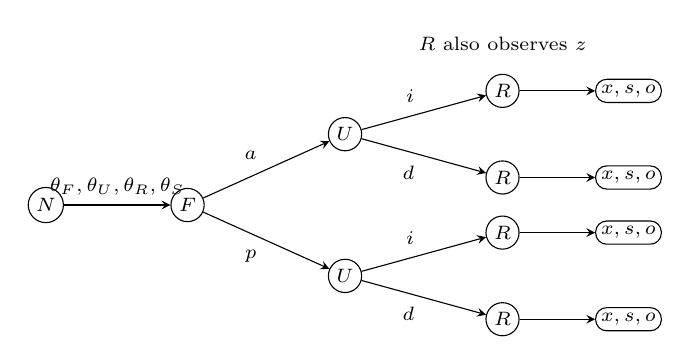
\begin{tikzpicture}[x=1cm,y=1cm,>=stealth,
  every node/.style={font=\scriptsize},
  decision/.style={circle,draw,inner sep=1.5pt},
  terminal/.style={rectangle,draw,rounded corners,inner sep=2pt}]
  \node[decision] (n) at (0,0) {$N$};
  \node[decision] (f) at (1.8,0) {$F$};
  \node[decision] (ua) at (3.8,0.9) {$U$};
  \node[decision] (up) at (3.8,-0.9) {$U$};
  \node[decision] (rai) at (5.8,1.45) {$R$};
  \node[decision] (rad) at (5.8,0.35) {$R$};
  \node[decision] (rpi) at (5.8,-0.35) {$R$};
  \node[decision] (rpd) at (5.8,-1.45) {$R$};
  \node[terminal] (tai) at (7.4,1.45) {$x,s,o$};
  \node[terminal] (tad) at (7.4,0.35) {$x,s,o$};
  \node[terminal] (tpi) at (7.4,-0.35) {$x,s,o$};
  \node[terminal] (tpd) at (7.4,-1.45) {$x,s,o$};
  \draw[->] (n) -- node[above] {$\theta_F,\theta_U,\theta_R,\theta_S$} (f);
  \draw[->] (f) -- node[above left] {$a$} (ua);
  \draw[->] (f) -- node[below left] {$p$} (up);
  \draw[->] (ua) -- node[above left] {$i$} (rai);
  \draw[->] (ua) -- node[below left] {$d$} (rad);
  \draw[->] (up) -- node[above left] {$i$} (rpi);
  \draw[->] (up) -- node[below left] {$d$} (rpd);
  \draw[->] (rai) -- (tai);
  \draw[->] (rad) -- (tad);
  \draw[->] (rpi) -- (tpi);
  \draw[->] (rpd) -- (tpd);
  \node at (5.8,2.05) {$R$ also observes $z$};
\end{tikzpicture}
\caption{Extensive-form skeleton of the signaling game. Nature draws private
types; $F$ signals first, $U$ responds, and $R$ acts after observing both public
messages and the noisy public signal $z$.}
\label{fig:signaling-tree}
\end{figure}

\subsection{Cheap Talk and Pooling}
\label{subsec:cheap-talk-pooling}

Consider the cheap-talk cost structure in which $c_{\theta_F}(a)=c_{\theta_F}(p)=0$
for both governance types. Let $\Delta_F>0$ be the firm's ontological premium
from inducing user investment under anthropomorphic marketing. Let $B_{\theta_U}$
be the user's immediate benefit from investment and $H_{\theta_U}$ the expected
future harm from mistaken investment. Let $K_{\theta_R}$ be the regulator's cost
of inspection or sanction under bandwidth type $\theta_R$. The pooling region is
defined by three inequalities:
\[
\Delta_F>0,\qquad
B_{\theta_U}-\pi(\mathsf{L})H_{\theta_U}>0,\qquad
K_{\theta_R}>\pi(\mathsf{L})D_R .
\]
The first inequality says that anthropomorphic marketing is privately profitable
when users invest. The second says that each user type finds investment
privately optimal under the prior, because the immediate benefit exceeds the
discounted expected harm. The third says that, under the prior, regulator
intervention is not worth its cost.

One PBE in this region is the following. Both firm types send $a$:
\[
\sigma_F(\mathsf{H},\theta_S)=\sigma_F(\mathsf{L},\theta_S)=a .
\]
Both user types invest after $a$:
\[
\sigma_U(a,\mathsf{V})=\sigma_U(a,\mathsf{N})=i .
\]
The regulator abstains after observing $(a,i,z_0)$ for a neutral public signal
$z_0$:
\[
\sigma_R(a,i,z_0,\theta_R)=o .
\]
Off path, users detach after $p$ and the regulator abstains unless the public
signal independently makes inspection payoff-positive. These off-path actions
are supported by beliefs assigning low probability to high governance after the
deflationary message.

On the equilibrium path, the firm's message contains no type information. For a
neutral public signal satisfying
$q(z_0\mid \mathsf{H})=q(z_0\mid \mathsf{L})$, Bayes' rule gives
\[
\begin{aligned}
\mu_R(\mathsf{H}\mid a,i,z_0)
&=
\frac{\pi(\mathsf{H})q(z_0\mid \mathsf{H})}
{\pi(\mathsf{H})q(z_0\mid \mathsf{H})+\pi(\mathsf{L})q(z_0\mid \mathsf{L})}
\\
&=\pi(\mathsf{H}).
\end{aligned}
\]
Likewise $\mu_R(\theta_F=\mathsf{L}\mid a,i,z_0)=\pi(\mathsf{L})$ and
$U$'s posterior after observing $a$ equals its prior over $\theta_F$. More
generally, a non-neutral $z$ can move $R$ from $\pi$ to $\pi_z$, but the
messages $(a,i)$ add no information beyond the public channel. Pooling therefore
does not mean that regulators never learn; it means that the firm's cheap-talk
signal does not force learning.

Given the off-path beliefs specified above and the payoff inequalities of the
pooling region, no player has a profitable unilateral deviation. A firm that deviates from $a$
to $p$ loses the ontological premium because users detach off path; it does not
buy a lower enforcement risk because $R$ abstains on the equilibrium path
already. A user who deviates from $i$ to $d$ gives up positive expected surplus
under the second inequality. A regulator who deviates from $o$ to $x$ or $s$
incurs expected cost exceeding expected gain under the third inequality. The
result is a cheap-talk equilibrium in the sense of Crawford and Sobel:
communication occurs, but it does not separate types \citep{crawford_sobel1982}.

\subsection{Audit-Trail Costs and Separation}
\label{subsec:audit-trail-separation}

The mechanism-design problem is to change the cost of the firm's signal. Suppose
anthropomorphic marketing is valid only when paired with an audit trail of
intensity $e$: evaluation records, capability logs, incident reports, and
regulator-readable documentation. Let the net benefit from being perceived as
high-governance be $G>0$. Let audit cost be $c_H(e)=k_H e$ for high-governance
firms and $c_L(e)=k_L e$ for low-governance firms, with
$0<k_H<k_L$. This is the single-crossing condition: the marginal cost of the
same signal is lower for the type that actually invested in governance. The
Spence-style separating interval is
\[
\frac{G}{k_L} \leq e \leq \frac{G}{k_H}.
\]
Above the lower threshold $e^\ast=G/k_L$, the low-governance type does not want
to imitate. Below the upper bound $G/k_H$, the high-governance type still wants
to signal. When $e$ lies in this interval, a separating PBE exists:
high-governance firms send audited anthropomorphic claims, low-governance firms send
deflationary claims, users condition investment on the audited signal, and
regulators update posteriors to one on the equilibrium path.

\begin{proposition}[Cheap talk and audit-trail separation]
\label{prop:cheap-talk-separation}
Under the cheap-talk cost structure above, pooling on anthropomorphic marketing
is a Perfect Bayesian Equilibrium and survives the Intuitive Criterion. Under
an audit-trail signal cost satisfying single crossing in $\theta_F$, there is a
separating Perfect Bayesian Equilibrium in which $m_F$ reveals the firm's
governance type.
\end{proposition}

\paragraph{Proof sketch.}
For the cheap-talk part, the strategy profile and beliefs specified above are
sequentially rational and Bayes-consistent on path. Under the off-path beliefs
assigning low probability to high governance after the deflationary message, the
Intuitive Criterion does not eliminate the equilibrium because the off-path
deflationary message is costless for both firm types and is not uniquely
profitable for the high-governance type; no type can be excluded as an
implausible sender of the
deviation. For the separating part, choose $e$ in the interval
$[G/k_L,G/k_H]$. High-governance firms receive $G-k_He\geq 0$ from sending the
audited signal, while low-governance firms receive $G-k_Le\leq 0$ and therefore
prefer the deflationary message. Bayes' rule then assigns posterior probability
one to $\mathsf{H}$ after the audited anthropomorphic signal and posterior
probability one to $\mathsf{L}$ after the unaudited deflationary signal. Given
those beliefs, users and regulators condition their actions on the revealed type.
The audit trail therefore converts an uninformative cheap-talk message into a
costly signal in the sense of \citet{spence1973}.

% !TEX root = ../arbitrage.tex
\section{Why Cheap Talk Persists}
\label{sec:cheap-talk}

Section~\ref{sec:bayesian} identifies pooling on anthropomorphic marketing as a Perfect Bayesian Equilibrium under cheap-talk cost. This section gives five structural reasons for the empirical persistence of that equilibrium. Each is matched to a parameter of the model so that the proposals in Section~\ref{sec:mechanism} can be read as targeted cost changes rather than as welfare exhortations.

\emph{Opacity.} The system-opacity parameter $\theta_S$ is private to the firm. Capability claims about a deployed model cannot be falsified by reading model outputs alone, because the same outputs are compatible with very different training procedures, evaluation regimes, and post-deployment monitoring. Opacity is the precondition for the firm's premium: where outsiders could costlessly verify $\theta_F$, the spread between anthropomorphic and deflationary positioning would collapse. This is the lemons logic of \citet{akerlof1970}: under one-sided private information, the market clears at a price that reflects the worst credible quality, except that here the relevant ``quality'' is a governance disposition rather than a physical attribute.

\emph{Verification bandwidth.} The third inequality of the pooling region, $K_{\theta_R}>\pi(\mathsf{L})D_R$, encodes the regulator's inspection cost relative to expected gain. A low-bandwidth regulator faces an absolute cost so high that abstention is dominant under the prior; even a high-bandwidth regulator may be priced out across the full product population. The condition that produces this state is not unique to AI. \citet{pasquale2015} documents an analogous structure in algorithmic finance and consumer scoring: the opacity of the regulated object combines with the bandwidth of the regulator to make inspection a scarce resource allocated by triage rather than by uniform application.

\emph{Asynchronous harms.} The user's payoff term $H_{\theta_U}$ enters discounted. The episodes in which a relational reading proves costly---deprecation, persona shifts, crisis-handling failures---are temporally separated from the initial attribution by intervals over which the user has already accrued $B_{\theta_U}$. Under standard hyperbolic or even exponential discounting, the inequality $B_{\theta_U}-\pi(\mathsf{L})H_{\theta_U}>0$ holds for a wider class of users than the time-zero risk calculation would suggest. Asynchrony is not a behavioural bug; it is the timing structure of the harm itself.

\emph{Fragmentation of affected parties.} Publics, journalists, intellectuals, and affected communities are folded into the noisy channel $z$ rather than modelled as autonomous players. This is not a normative claim that they lack standing; it is an institutional observation. Their costs of coordination are high, their access to inspection technology is uneven, and their incentives to invest in any particular case are individually small. Even when $z$ carries substantial information about $\theta_F$, regulators cannot treat it as binding without a procedural translation that the channel itself does not provide. The fragmentation result is closely related to the cheap-talk multiplicity of \citet{crawford_sobel1982}: with many would-be senders and a single noisy aggregator, the informative subset of equilibria is not selected for.

\emph{No penalty for inconsistency.} The cheap-talk cost structure sets $c_{\theta_F}(a)=c_{\theta_F}(p)=0$ for both governance types and---more importantly for this section---imposes no joint constraint across $m_F$. Marketing copy and policy documentation are produced under different audiences, different review processes, and different liability regimes. Inconsistency between them is not detected as a single offence; it is decomposed into two compliant statements at two different points of contact. The firm's premium $\Delta_F$ is rent earned precisely on this decomposition. Until the signal cost makes inconsistency itself sanctionable---the proposal of Section~\ref{subsec:sanctionable-inconsistency}---there is no parameter under the firm's control whose adjustment would close the spread.

\emph{Pooling is the market's stable terminal state.} These five structural conditions jointly explain why ethical appeals fail to dislodge the equilibrium. They do not fail because AI governance discourse lacks moral seriousness; they fail because moral seriousness is itself a zero-cost signal. Under the cheap-talk cost structure, a declaration of ``responsible AI'' is formally indistinguishable from any other message at $c_{\theta_F}(a)=0$: both governance types can issue it at the same cost, so it contains no type information and moves no posterior. The equilibrium is not a moral failure. It is the unique stable outcome of the incentive structure as currently constituted, even if the outcome is welfare-reducing in aggregate. A firm that unilaterally forgoes the ontological premium $\Delta_F$---that chooses deflationary marketing across all channels and forfeits the user investment it would otherwise attract---loses revenue it cannot recover from customers who face no such constraint. Market selection eliminates non-arbitraging firms not because restraint is penalized directly, but because the competitor who retains $\Delta_F$ captures the market segment that the restrained firm vacates. The implication is precise: \emph{the market does not reward non-exploitation; it eliminates firms that do not arbitrage}. The mechanisms in Section~\ref{sec:mechanism} respond to this implication by changing the cost parameters rather than appealing to the conscience of players who are already acting rationally.

\begin{table}[t]
\centering
\scriptsize
\setlength{\tabcolsep}{3pt}
\renewcommand{\arraystretch}{1.2}
\begin{tabular}{@{}p{2.7cm}p{2.2cm}p{2.7cm}@{}}
\toprule
\textbf{Structural Condition} & \textbf{Model Parameter} & \textbf{Intervention (\S\ref{sec:mechanism})} \\
\midrule
No penalty for inconsistency & $c_{\theta_F}(a)=c_{\theta_F}(p)=0$ & Sanctionable inconsistency \\
Opacity & $\theta_S$ private to firm & Costly third-party audits \\
Verification bandwidth & $K_{\theta_R}>\pi(\mathsf{L})D_R$ & Auditable records \\
Asynchronous harms & $H_{\theta_U}$ enters discounted & Evidentiary lag priced \\
Fragmentation & $z$ noisy, high coord.\ cost & Aggregation cost lowered \\
\bottomrule
\end{tabular}
\caption{Mapping of structural persistence conditions to model parameters and cost-imposition mechanisms.}
\label{tab:condition-map}
\end{table}

% !TEX root = ../arbitrage.tex
\section{Mechanism Design: Equilibrium Redesign}
\label{sec:mechanism}

The preceding sections identify a precise failure mode. Under cheap-talk costs,
anthropomorphic marketing can pool across governance types, users rationally
invest under the prior, and regulators abstain when inspection is too costly.
The policy implication is not that regulators should decide whether AI systems
are persons. It is that the public signal environment should be redesigned so
that inconsistent ontological claims no longer remain costless. In
mechanism-design terms, the problem is to make truthful revelation of $\theta_F$ incentive
compatible rather than to ask firms to volunteer it \citep{myerson1979}.

The proposals below therefore alter the game in Section~\ref{sec:bayesian} at
three different points: the cost of inconsistent messages, the cost of
anthropomorphic claims, and the regulator's cost of verification. Each proposal
has the same structure. It modifies a model parameter, states the equilibrium
shift induced by that modification, and points to an existing legal form that
establishes feasibility. The analogs are not claims that current doctrine already
solves AI ontology. They show that adjacent legal systems already know how to
attach consequences to half-truths, require substantiation before marketing, and
make internal records available to oversight institutions.

\subsection{Sanctionable Inconsistency}
\label{subsec:sanctionable-inconsistency}

The first intervention treats the firm's public message as a joint object rather
than as two isolated texts. In the cheap-talk model, marketing can send $a$
while policy and liability documents send $p$, with no cost assigned to the
inconsistency. A sanctionable-inconsistency rule would require firms to maintain
a claim register linking outward-facing marketing, safety statements, terms of
service, incident disclosures, and liability positions. If the firm represents
the system as agentic, caring, autonomous, or safety-critical in one channel
while denying the legal significance of the same representation in another,
that cross-channel inconsistency becomes independently sanctionable.

\paragraph{Parameter changed.}
This adds a penalty term $S_I$ to the firm's payoff for inconsistent message
pairs. If $\rho_R$ is the probability that $R$ detects or accepts proof of the
inconsistency, the cheap-talk premium becomes
\[
\Delta_F-\rho_R S_I .
\]
Pooling on anthropomorphic marketing is no longer profitable when
$\rho_R S_I>\Delta_F$. The rule therefore attacks the exact term that made
arbitrage attractive: the rent earned from pricing the system as agent in the
user channel while pricing it as tool in the liability channel.

\paragraph{Equilibrium shift.}
The induced shift is not necessarily full separation. It can also operate by
constraining off-path beliefs. If $R$ observes an inconsistent pair $(a,p)$,
then the admissible posterior places greater mass on $\theta_F=\mathsf{L}$ or
on high opacity $\theta_S$. Firms anticipating that posterior either harmonize
their claims or choose the deflationary message across channels. In both cases,
the cheap-talk pooling equilibrium loses its most valuable deviation: firms can
no longer take the marketing upside of $a$ while preserving the liability
downside of $p$.

\paragraph{Existing-law analog.}
The legal analog is familiar. FTC Act Section 5 treats unfair or deceptive acts
or practices as sanctionable, and advertising-substantiation doctrine already
asks whether the net impression of a claim is misleading to the relevant
audience. Securities antifraud rules provide the parallel logic for investor
communications: Rule 10b-5 targets material misstatements and omissions that
make statements misleading in context. The proposed rule imports that
cross-document logic without importing securities doctrine wholesale. Its point
is narrower: a firm should not be able to produce one ontology for users and an
incompatible ontology for adjudicators without paying a regulatory price.

\subsection{Costly Signaling Through Third-Party Audits}
\label{subsec:costly-signaling-audits}

The second intervention makes anthropomorphic or agency-adjacent marketing a
costly signal. A firm may still describe a system as a companion, agent,
co-worker, tutor, or safety-critical assistant, but only after a qualified third
party verifies the governance conditions that make such a claim non-misleading:
evaluation coverage, red-team results, escalation pathways, incident-response
capacity, model-update controls, and post-deployment monitoring. The audit does
not certify consciousness or moral status. It certifies the institutional
conditions behind the claim.

\paragraph{Parameter changed.}
This implements the audit-trail cost from Proposition~\ref{prop:cheap-talk-separation}.
Let audit intensity be $e$, with $c_H(e)=k_He$ for high-governance firms and
$c_L(e)=k_Le$ for low-governance firms, where $0<k_H<k_L$. The separating
interval derived in Section~\ref{subsec:audit-trail-separation} is
\[
\frac{G}{k_L}\leq e\leq \frac{G}{k_H}.
\]
Above the lower threshold, low-governance firms cannot profitably mimic. Below
the upper threshold, high-governance firms can still afford to signal. The
regulator's task is therefore not to maximize audit burden. It is to set $e$ in
the interval where signal cost separates types.

\paragraph{Equilibrium shift.}
The shift is from pooling to separating PBE. High-governance firms send audited
anthropomorphic claims; low-governance firms either invest in governance until
their cost curve changes or use deflationary marketing. Users can then condition
investment on an informative signal rather than on undisciplined warmth in
product copy. Regulators can condition abstention on the audit result rather
than on an unverified prior. This is the Spence logic of costly signaling
applied to AI governance claims \citep{spence1973}; it also follows the
advertising-as-signal insight that market messages become informative only when
false messages are sufficiently expensive \citep{milgrom_roberts1986}.

\paragraph{Existing-law analog.}
The analogs are pharmaceutical efficacy review and food-labeling controls. In
both domains, public-facing claims are not left entirely to seller narrative:
claims about therapeutic effect or product identity must be supported before
they can be used to shape consumer reliance. The same design can be translated
to AI without pretending that AI companionship is a drug or a food. The common
institutional pattern is substantiation-before-reliance: when a claim predictably
changes how vulnerable users act, the law may require evidence before allowing
the claim to be marketed at scale.

\subsection{Auditable Records for Regulator-Readable Verification}
\label{subsec:auditable-records}

The third intervention reduces the regulator's verification cost by requiring
append-only, regulator-readable records tied to capability and relational
claims. Records should include the claim identifier, model version, relevant
evaluation suite, deployment date, material model updates, safety interventions,
known incident classes, and the internal owner responsible for the claim. The
point is not to publish every interaction or expose user data. It is to create a
durable evidentiary substrate that lets $R$ test whether a public claim remained
true across model updates and incidents.

\paragraph{Parameter changed.}
In the pooling condition from Section~\ref{subsec:cheap-talk-pooling}, the
regulator abstains when $K_{\theta_R}>\pi(\mathsf{L})D_R$. Auditable records
lower $K_{\theta_R}$ and can increase expected detection value $D_R$:
\[
K'_{\theta_R}=K_{\theta_R}-\lambda,\qquad
D'_R=D_R+\eta .
\]
When $K'_{\theta_R}\leq \pi(\mathsf{L})D'_R$, inspection becomes sequentially
rational. Records also improve the public channel $z$ by giving journalists,
researchers, and civil society a procedural object to demand or contest, rather
than leaving them to infer governance quality from outputs alone.

\paragraph{Equilibrium shift.}
The shift is from abstention under unverifiable priors to credible inspection.
Once firms know that claims are tied to records, a low-governance firm faces a
higher expected cost from exaggeration even if it is not inspected in every
case. This complements the first two proposals. Sanctionable inconsistency tells
firms which cross-channel contradictions will be penalized; costly signaling
tells firms what evidence is required before making anthropomorphic claims;
auditable records make both rules administrable over time.

\paragraph{Existing-law analog.}
Several regulatory systems already use this form. GDPR Article 30 requires
records of processing activities. Sarbanes-Oxley Section 404 links public
reporting to internal control over financial reporting. EU AI Act Article 12
requires logging capabilities for high-risk AI systems. None is a complete
template for relational AI governance, but each shows the same institutional
move: private organizations must produce internal records in a form that public
oversight can inspect. That is the rule-of-law function of documentation in
complex technical systems \citep{hadfield2017rules}.

Taken together, these interventions change the equilibrium rather than merely
condemning the equilibrium. Sanctionable inconsistency taxes contradictory
messages. Costly audits create a separating signal for $\theta_F$. Auditable
records lower $K_{\theta_R}$ and make public signal $z$ less noisy. The result
is not metaphysical settlement. It is a governance design in which firms remain
free to choose their ontology, but not to arbitrage incompatible ontologies
across audiences at zero cost.


\appendix
\section{Isabelle/HOL Formalization Appendix}
\label{app:isabelle}

This appendix outlines the formal verification of the signaling game equilibria using the Isabelle/HOL proof assistant. The complete source code of the formalization is available in the \texttt{isabelleHOL/} directory, specifically within the theory file \texttt{Ontological\_Arbitrage.thy}.

We formalize the game-theoretic structure by defining explicit ex-post payoffs for the three players (Firm, User, and Regulator) and computing expected payoffs via uniform probability weights over the finite action and type spaces. Under these generalized definitions, we prove the existence of the Perfect Bayesian Equilibria (PBE) for both the cheap-talk and the audit-trail game variants:
\begin{itemize}
    \item \textbf{Theorem \texttt{proposition\_\allowbreak{}1\_\allowbreak{}cheap\_\allowbreak{}talk\_\allowbreak{}pooling\_\allowbreak{}pbe}} formalizes the cheap-talk pooling equilibrium where both high- and low-governance firms pool on the anthropomorphic message, and receivers play their prior-based optimal actions (Invest and Abstain, respectively). We prove this profile survives a limited variant of the Cho-Kreps Intuitive Criterion.
    \item \textbf{Theorem \texttt{proposition\_\allowbreak{}1\_\allowbreak{}separating\_\allowbreak{}pbe}} formalizes the audit-trail separating equilibrium supported by the single-crossing audit cost structure. High-governance firms separate by incurring the audit trail cost, while low-governance firms find mimicry unprofitable and choose the deflationary message.
\end{itemize}
All theorems, definitions, and supporting lemmas are fully checked and verified by Isabelle/HOL without any unresolved assumptions or proofs.


\bibliography{arbitrage}

\end{document}
